\section{Entropy, Relative Entropy, Mutual Information}
$X\sim f(x)$, where $f(x)$ is the PDF.
$$h(X)=-\int_x f(x)\log f(x)dx=\mathbb{E}_{X\sim f(x)}\left[-\log f(x)\right]$$
\begin{align*}
h(X) & =-\int_x f(x)\log f(x) \dx \text{ bits} \\
&= -\int_x f(x)\textcolor{red}{\ln} f(x) \dx \text{ nats}
\end{align*}
不同于离散型随机变量 $0\leq H(X) \leq \log |\mathcal{X}|$有界, 连续型随机变量 $h(X)$ 无界. $h(X)$ 是反常积分, 可以 $<0$, 也可能不存在($\to \infty$). 但$h(X)$ 仍可以反映$X$ 的不确定性, $h(X)$ 越大, $X$ 的不确定性越大.

\begin{example}
$X\sim \text{Unif}(a, b)$, $f(x)=\dfrac{1}{b-a}$, $a\leq x\leq b$.
$$h(X)=-\int_a^b \dfrac{1}{b-a}\log \dfrac{1}{b-a} \dx=\log(b-a)$$
For example, when $a=0, b=0.5$, $h(X)=\log 0.5=-1<0$.
\end{example}

\begin{example}
$X\sim\mathcal{N}(\mu, \sigma^2)$, $f(x)=\dfrac{1}{\sqrt{2\pi}\sigma}\exp\left(-\dfrac{(x-\mu)^2}{2\sigma^2}\right)$.
\begin{align*}
h(X) &= -\int_{-\infty}^{\infty} \dfrac{1}{\sqrt{2\pi}\sigma}\exp\left(-\dfrac{(x-\mu)^2}{2\sigma^2}\right)\ln \dfrac{1}{\sqrt{2\pi}\sigma}\exp\left(-\dfrac{(x-\mu)^2}{2\sigma^2}\right) \dx \\
&= \int_{-\infty}^{\infty} \dfrac{1}{\sqrt{2\pi}\sigma}\exp\left(-\dfrac{(x-\mu)^2}{2\sigma^2}\right)\left( \ln\left(\sqrt{2\pi}\sigma\right) + \dfrac{(x-\mu)^2}{2\sigma^2}\right) \dx \\
&= \dfrac{1}{2\sigma^2}\int_{-\infty}^{\infty} \dfrac{1}{\sqrt{2\pi}\sigma}(x-\mu)^2\exp\left(-\dfrac{(x-\mu)^2}{2\sigma^2}\right) \dx \\
&\quad + \ln\left(\sqrt{2\pi}\sigma\right) \int_{-\infty}^{\infty} \dfrac{1}{\sqrt{2\pi}\sigma}\exp\left(-\dfrac{(x-\mu)^2}{2\sigma^2}\right) \dx
\end{align*}
For the first part(variance):
$$\Var(X)=\mathbb{E}\left[(X-\mathbb{E}(X))^2\right]=\int_{-\infty}^{\infty} (x-\mu)^2 \dfrac{1}{\sqrt{2\pi}\sigma}\exp\left(-\dfrac{(x-\mu)^2}{2\sigma^2}\right) \dx=\sigma^2$$
For the second part(integral of PDF):
$$\int_{-\infty}^{\infty} \dfrac{1}{\sqrt{2\pi}\sigma}\exp\left(-\dfrac{(x-\mu)^2}{2\sigma^2}\right) \dx=1$$
So put them into the equation:
$$h(X)=\dfrac{1}{2\sigma^2}\sigma^2 + \ln\left(\sqrt{2\pi}\sigma\right)=\dfrac{1}{2}\textcolor{red}{\ln}(2\pi e\sigma^2) \textcolor{red}{\ nats} =\dfrac{1}{2}\textcolor{red}{\log}(2\pi e\sigma^2) \textcolor{red}{\ bits} $$
\end{example}

\begin{definition}
Joint Differential Entropy: $X_1,\ldots,X_n\sim f(x_1,\ldots,x_n)$, then
$$h(X_1,\ldots,X_n)=-\int_{x^n} f(x^n)\log f(x^n) \dx^n$$
\end{definition}

\begin{definition}
Conditonal Differential Entropy:
\begin{align*}
h(X|Y) &= -\int_{x,y} f(x,y)\log f(x|y) \dx \dy \\
&= h(X,Y)-h(Y)
\end{align*}
\end{definition}

\begin{definition}
Relative Entropy(KL Divergence): 为了保证连续性质, 定义 $0\log\dfrac{0}{0}=0$.
\begin{align*}
-D(f\|g) &= -\int_x f(x)\log \dfrac{f(x)}{g(x)} \dx \\
&= \mathbb{E}_{X\sim f(x)}\left[\log \dfrac{g(X)}{f(X)}\right] \\
&\leq \log \left(\mathbb{E}_{X\sim f(x)}\left[\dfrac{g(X)}{f(X)}\right]\right) \\
&= \log \left(\int_x f(x) \dfrac{g(x)}{f(x)} \dx\right) \\
&= \log \left(\int_x g(x) \dx\right) = \log 1 \\
&= 0
\end{align*}
i.e. $D(f\|g)\geq 0$, and $D(f\|g)=0$ if and only if $f=g$.
\end{definition}

\begin{definition}
Mutual Information:
$$I(X;Y)=\int_{x,y} f(x,y)\log \dfrac{f(x,y)}{f(x)f(y)} \dx \dy $$
Similarly with discrete case:
$$I(X;Y)=h(X)-h(X|Y)=h(Y)-h(Y|X)=h(X)+h(Y)-h(X,Y)$$
由于 $I(X;Y) = KL(f(x,y)\|f(x)f(y)) \geq 0$, 所以 $h(X) \geq h(X|Y)$, i.e. conditioning reduces entropy仍成立.
\end{definition}

\begin{proposition}
在指定范围$[a,b]$内的所有分布中, 若对分布没有限制, 则当且仅当均匀分布$X\sim \text{Unif}(a,b)$时熵最大$\log (b-a)$. \\
proof: Let $u(x)$ be the PDF of Unif$(a,b)$, $f(x)$ be the PDF of any other distribution in $[a,b]$. Then
\begin{align*}
0 &\leq D\left(f\|u\right) = \int_{a}^{b}f(x)\ln \dfrac{f(x)}{u(x)} \dx \\
&= \int_{a}^{b}f(x)\ln u(x) \dx - \int_{a}^{b}f(x)\ln f(x) \dx \\
&= \ln(b-a) - h(f) \\
&= h(u) - h(f)
\end{align*}
\end{proposition}

\begin{proposition}
$\forall C\in \mathbb{R}$, $h(X+C)=h(X)$. 熵衡量不确定性, 只改变均值, 概率(不确定性)不变.
\end{proposition}

\begin{proposition} \textcolor{blue}{书上似乎有问题? 积分换元漏掉了绝对值导致的正负号变化.}
$$h(aX) = h(X)+\log |a|$$
由change of variable: $f(\mathbf{Y})=f(\mathbf{X})\left|\dfrac{\partial \mathbf{X}}{\partial \mathbf{Y}}\right|$, 可得: \\
Let $Y=aX\Rightarrow f_Y(y)=f_X(x)\dfrac{1}{|a|}=\dfrac{1}{|a|}f_X\left(\dfrac{y}{a}\right)$.
\begin{align*}
h(Y) &= -\int_y f_Y(y)\log f_Y(y) \dy \\
&= -\int_y \dfrac{1}{|a|}f_X\left(\dfrac{y}{a}\right)\log \dfrac{1}{|a|}f_X\left(\dfrac{y}{a}\right) \dy \\
&= \textcolor{blue}{\dfrac{a}{|a|}}\cdot \left(-\int_x f_X(x)\log \dfrac{1}{|a|}f_X(x) \dx \right) \\
&= \textcolor{blue}{(-1)^{\mathbb{I}_{a<0}}}\left(h(X)+\log |a| \right)
\end{align*}
$a>1$, $h(aX)>h(X)$, $0<a<1$, $h(aX)<h(X)$.
\end{proposition}

\begin{proposition}
由上一个命题, 拓展到向量: $\mathbf{x}\in\mathbb{R}^n, \mathbf{A}\in\mathbb{R}^{n\times n}$, then
$$h(\mathbf{Ax})=h(\mathbf{x})+\log |\det (\mathbf{A})|$$
\end{proposition}

\begin{proposition}
离散与连续的关系:
\begin{figure}[htbp]
    \centering
    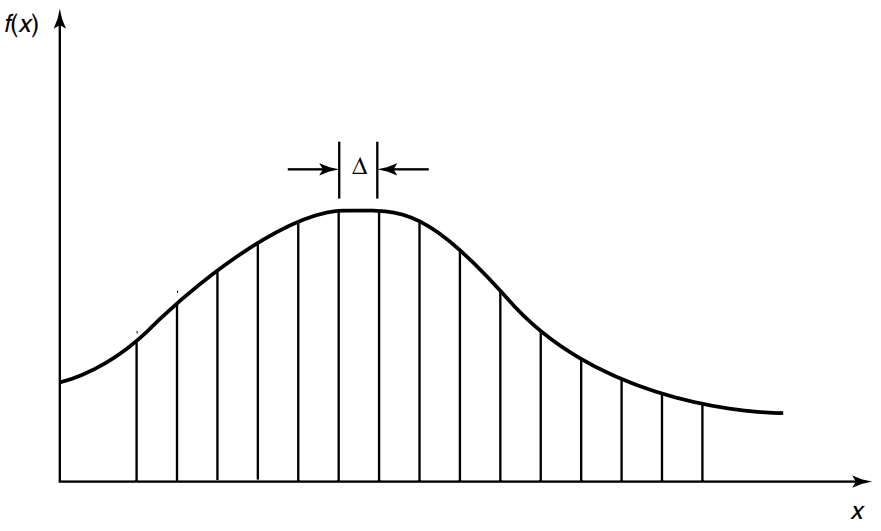
\includegraphics[width=0.66\textwidth]{./figures/chapter6/quantization.png}
\end{figure}
\end{proposition}
由积分中值定理: $f(x)$在$[a,b]$上连续, 则$\exists \epsilon\in[a,b]$, s.t. $$(b-a)f(\epsilon)=\int_a^b f(x) \dx$$
将连续型随机变量进行量化, 每$\Delta$为一个 bin / block, 记第i个bin为区间$[i\Delta, (i+1)\Delta]$, 则 $\exists x_i\in [i\Delta, (i+1)\Delta]$, s.t.
$$p_i=f(x_i)\cdot\Delta = \int_{i\Delta}^{(i+1)\Delta} f(x) \dx$$
Then we construct the quantization random variable $X^{\Delta}$, s.t. $X^{\Delta}=x_i$ with probability $p_i$. Then we have:
\begin{align*}
H(X^{\Delta}) &= -\sum_{i=-\infty}^{+\infty} p_i\log p_i \\
&= -\sum_{i=-\infty}^{+\infty} f(x_i)\Delta\log \left(f(x_i)\Delta\right) \\
&= -\sum_{i=-\infty}^{+\infty} f(x_i)\Delta\log f(x_i) -  \sum_{i=-\infty}^{+\infty} \underbrace{f(x_i)\Delta}_{p_i}\log \Delta \\
&\to -\int_{-\infty}^{+\infty} f(x)\log f(x) \dx - \log \Delta \\
&= h(X) - \log \Delta
\end{align*}
如果函数 $f(x)\log f(x)$黎曼可积, 则当$\Delta\to 0$时
$$-\sum_{i=-\infty}^{+\infty} f(x_i)\Delta\log f(x_i)\to -\int_{-\infty}^{+\infty} f(x)\log f(x) \dx$$
所以有结论
$$H(X^{\Delta}) + \log \Delta \to h(X), \text{ as } \Delta\to 0$$
如果在$[a,b]$上, 用$n$个bit进行量化, 即$\Delta = 2^{-n}$, 则
$$h(X) = H(X^{\Delta}) - n$$